% !TeX root = ../main.tex
% %%%%%%%%%%%%%%%%%%%%%%%%%%%%%%%%%%%%%%%%%%%%%%%%%%%%%%%%%%%%%%%%%%%%%%%%%%%%%%
% Monitoring
\chapter{Monitoring}
\label{chap:monitoring}

This chapter explains the whole process of monitoring, from compilation to error detection. First, the overall process of compilation is explained (\autoref{sec:runtimemonitoring}), then the generated file and some of its specifications are described (\autoref{sec:generatedfile}), and finally, the shown error messages are illustrated (\autoref{sec:errormessages}).


% ------------------------------------------------------------------------------
% Runtime Monitoring
\section{Runtime Monitoring}
\label{sec:runtimemonitoring}

After writing all the desired robotic systems specifications, the file needs to be compiled to generate the monitoring python file. Currently, to compile a specification file, one has to do it through the console under the same directory of the \textit{language.py} file. As for the command:

\texttt{python language.py properties.txt /home/ros\_workspace/src/my\_pkg/src}

The \textit{language.py} file needs to be run as a python file and be given as arguments:

\begin{enumerate}
    \item The specifications file name, and in case it is not in the same directory as the \textit{language.py} file, give its absolute path.
    \item The expected absolute path of the generated python monitoring file.
\end{enumerate}

The given directory for the generated file should be under a ROS workspace for the compilation to succeed. This is because, during the compilation, access to information like the available ROS messages might be necessary.

The monitoring file can now run as an independent ROS node, integrated into a launch file, or using rosrun in the console to execute it.


% ------------------------------------------------------------------------------
% Generated File
\section{Generated File}
\label{sec:generatedfile}

Declare the needed subscribers and use ApproximateTimeSynchronizer to call the callback function. The ApproximateTimeSynchronizer synchronizes messages by their timestamp and if they do not have a header, use the ROS time.

The callback function is called every time a new message from one of the subscribers is received. The callback function saves the relevant information for property checking in a global variable. This information serves as a current "screenshot" of the simulation representing its current state.

The node executes a loop at a delineated rate, doing the following tasks. 

Check if the defined simulation timeout time has reached. 

Save the current simulation state obtained by the callback function. This is necessary because the callback function is called at fluctuating rates, and we want to save multiple "screenshots" of the simulation at the loop fixed rate to make correlations with past states. 

Verify the properties using the saved states and calling each created function. An independent function with the necessary computations for verifying the property is defined for each base property.


% ------------------------------------------------------------------------------
% Error Messages
\section{Error Messages}
\label{sec:errormessages}

An error message starts by stating the line in the specification file which resulted in an error and showing the specification itself.

Afterward, the value at the time of failure of all the variables present at the specification is shown.

\begin{figure}[h]
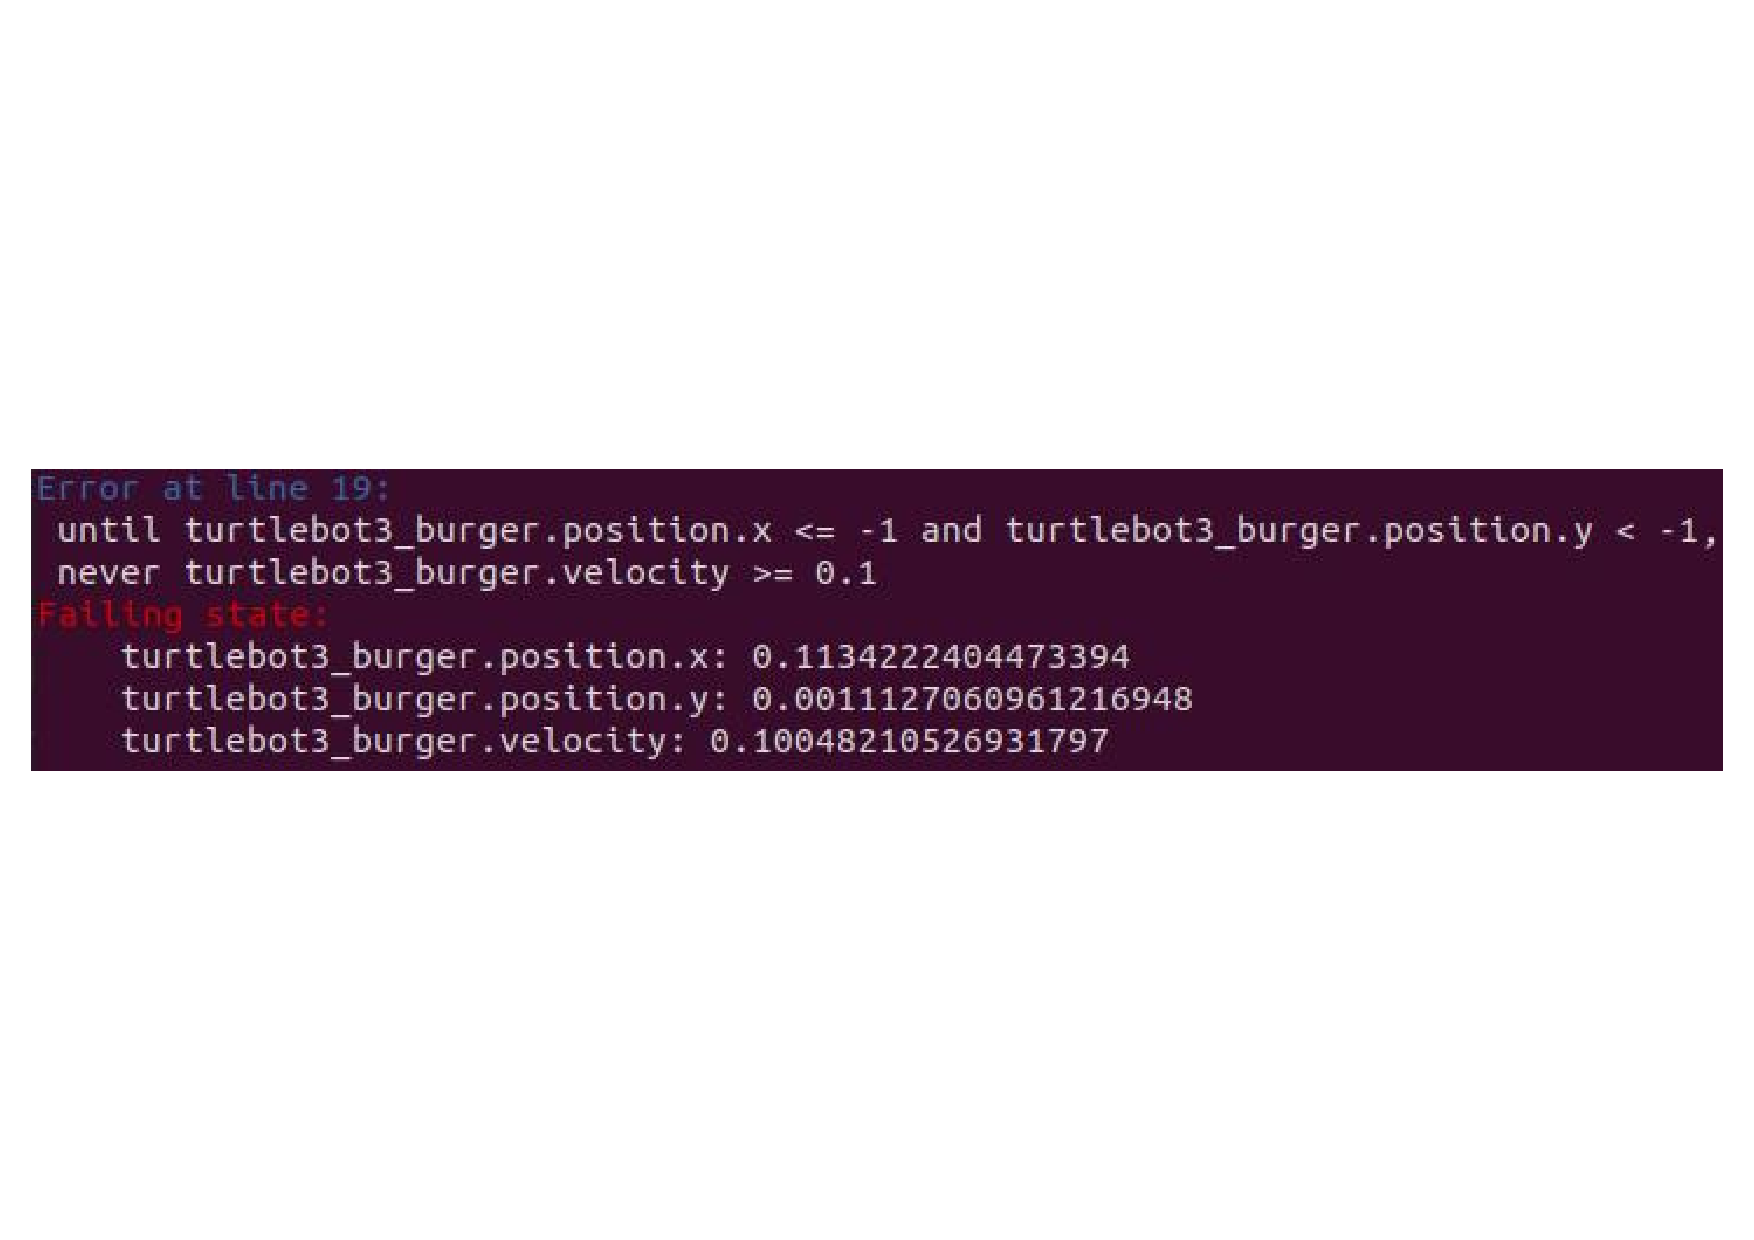
\includegraphics[width=\textwidth]{images/error_message.pdf}
\caption{Example of an error message.} \label{fig2}
\end{figure}